\documentclass[12pt,a4paper]{ctexart}
\usepackage{titlesec}%调节标题格式
\titleformat*{\section}{\zihao{3}\bfseries\centering}
\titleformat*{\subsection}{\zihao{4}\bfseries}
\titleformat*{\subsubsection}{\zihao{4}\bfseries}
\usepackage[utf8]{inputenc}
\usepackage[T1]{fontenc}
\usepackage{amsmath}
\usepackage{pifont}
\renewcommand\thefootnote{\ding{\numexpr171+  \value{footnote}}}
\newcommand\Emph{\textbf}
\usepackage{amssymb}
\usepackage{makeidx}
\usepackage{graphicx}
\graphicspath{{figures/}}%figures环境
\usepackage{float}
\usepackage{booktabs}
\usepackage{multirow}
\usepackage{tabularray}
\UseTblrLibrary{diagbox}%表格首行首列斜线
\UseTblrLibrary{amsmath}
\usepackage[section]{placeins}
\usepackage{geometry}
\geometry{hcentering}
\geometry{left=2.5cm,right=2.5cm,top=3cm,bottom=3cm}%设置左右页边距
\setcounter{secnumdepth}{4}%设置目录标题深度为4
\setcounter{tocdepth}{4}
\usepackage{color}
\usepackage{hyperref}%加高亮框框,但容易和其他包冲突,故放在后面
\begin{document}
	\begin{titlepage}
		\centering
		\zihao{1}土力学\cite{钱建固2015}期末\protect\footnotemark%脚注符号与内容分开,这是脚注符号
		\\
		\vspace*{\baselineskip}
		\zihao{-4}by:一只学土木的鼠鼠
		\footnotetext{edited by \LaTeX}%脚注符号与内容分开,这是脚注内容
		\newpage
	\end{titlepage}
	\thispagestyle{empty}%不标出页码
	\newpage
	\thispagestyle{empty}%放在插入目录前
	\tableofcontents
	\thispagestyle{empty}
	\setcounter{page}{0}
	\newpage
	\setcounter{secnumdepth}{-1}%设置section章节不标号
	\section{第一章:土的物理性质及工程分类}
	\subsection{两个经典问题}
	\begin{enumerate}
		\item 什么是土力学:
		
		描述土的\textcolor{red}{变形、强度和渗透特性}以及与此有关工程问题的一门学科
		\item 土的特点:
		
		\textcolor{red}{碎散性、三相性、天然性}
	\end{enumerate} 
	\subsection{土的颗粒特征}
	\textcolor{cyan}{土的颗粒级配}:土的颗粒大小及其组成情况,通常用土中各个不同粒组的相对含量(各粒组干土质量的百分比来表示)。
	
	在累计曲线上有两个非常重要的系数,可以描述土的级配的指标:
	
	\textcolor{cyan}{不均匀系数}
		\begin{equation}
		C_u=\frac{d_{60}}{d_{10}}
		\end{equation}
	
	\textcolor{cyan}{曲率系数}
		\begin{equation}
		C_s=\frac{d^2_{30}}{d_{60} d_{10}}
		\end{equation}
	
	式中,$d_{10}$、$d_{30}$、$d_{60}$分别相当于累计百分含量为10\%、30\%,60\% 的粒径。
	
	工程中,\textcolor{red}{当同时满足$C_u\geqslant 5$和$C_s=1\textasciitilde 3$时},土的级配良好,为不均匀土。
	
	\subsection{土的三相比例指标(计算重点)}
	土的三相图是解决这类计算题的关键,如下图所示
		\begin{figure}[htp]
			\centering
			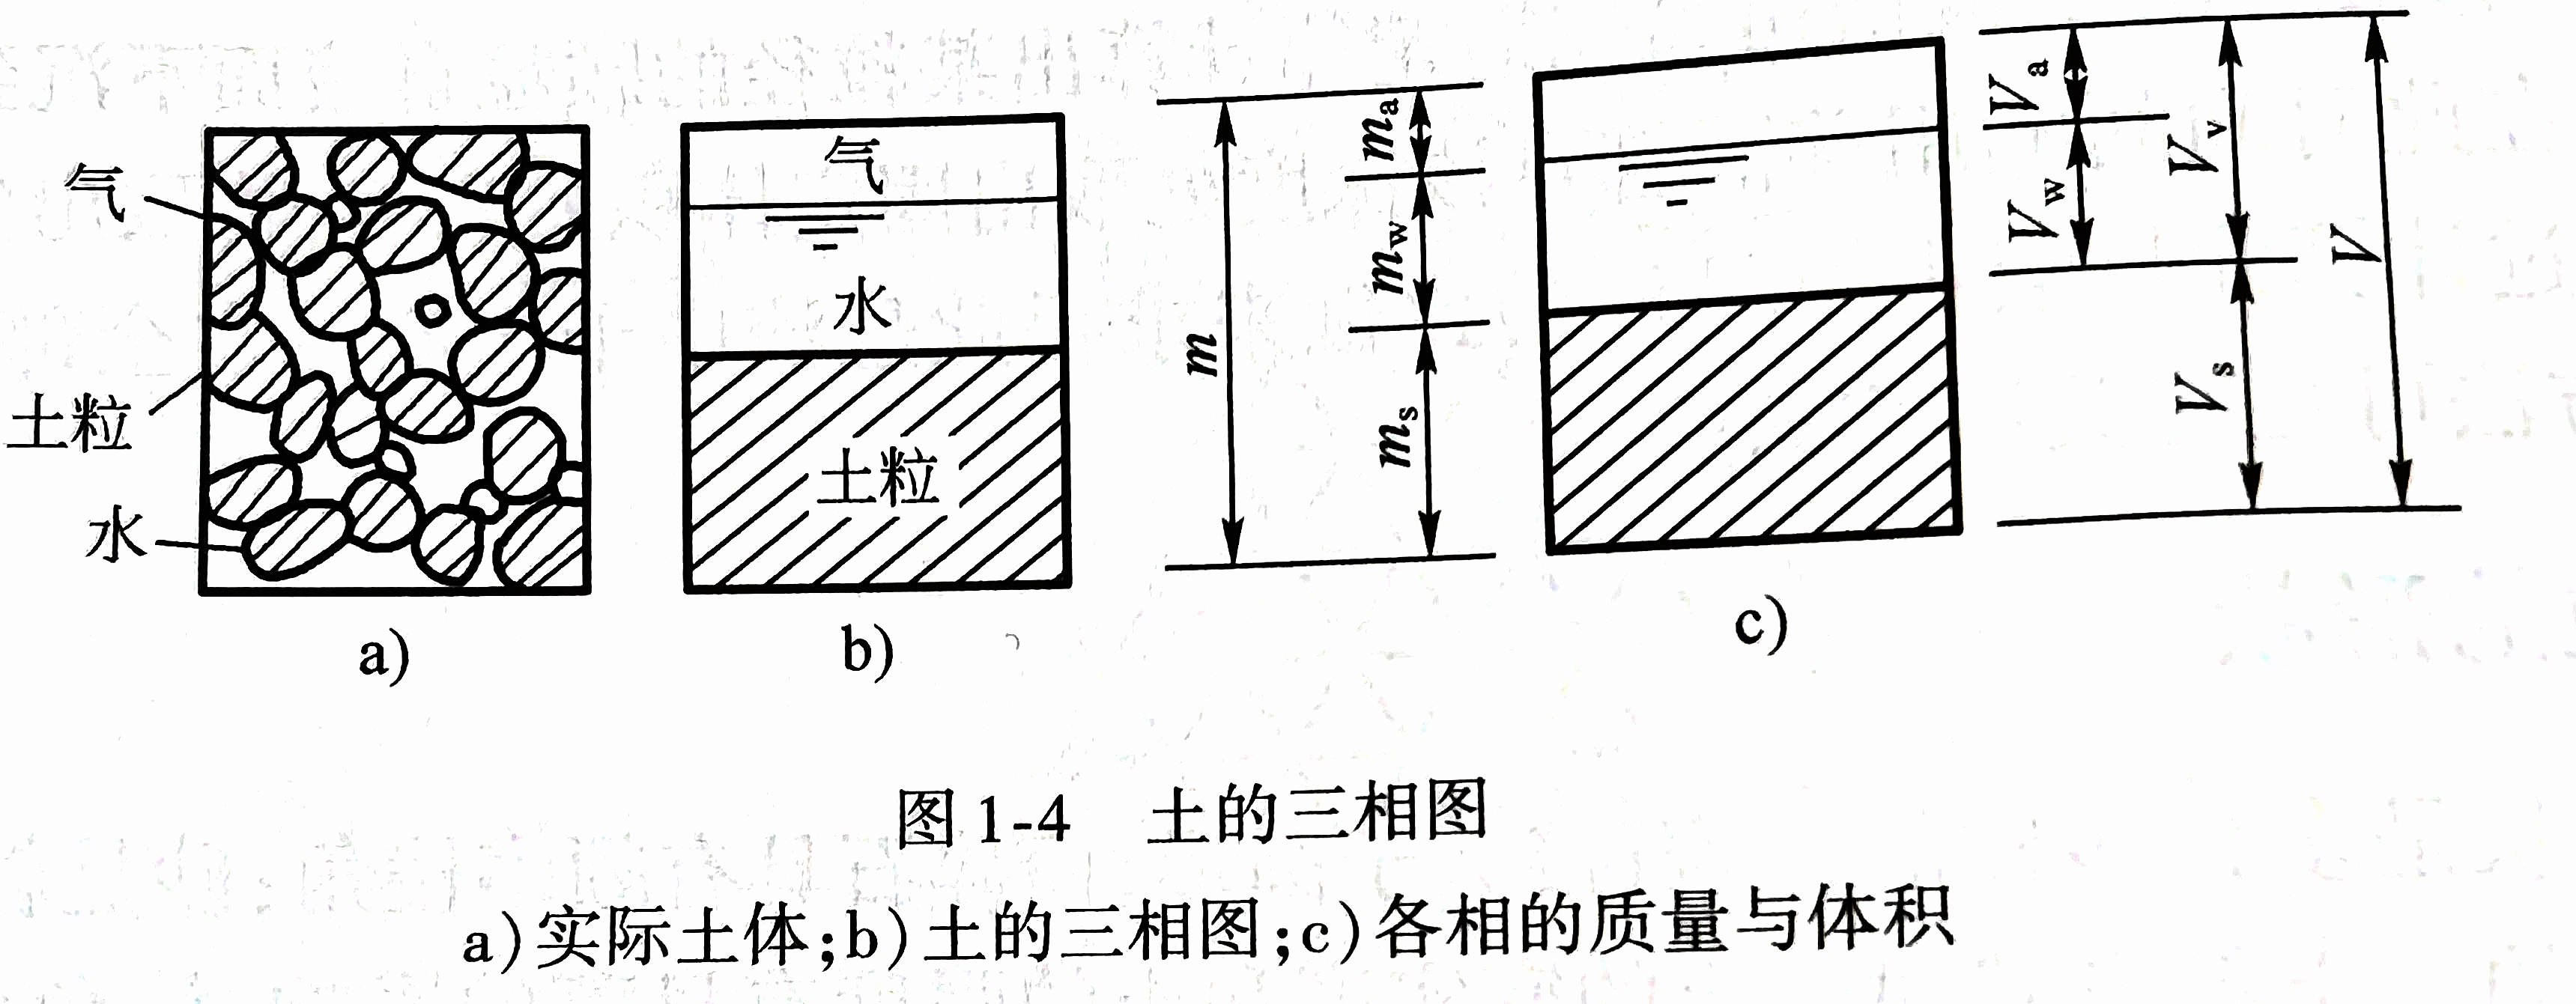
\includegraphics[width = 10cm ]{sxt}
		\end{figure}
	
	土的物理性质指标分为两类:
	
	1. 直接通过实验测定的有:
	
	\textcolor{cyan}{土的密度($\rho$)}
		\begin{equation}
			\rho=\frac{m}{V}=\frac{m_s+m_w}{V_s+V_w+V_a}
		\end{equation}
	单位为$g/cm^3$
	
	\textcolor{cyan}{土的比重($G_s$)}
			\begin{equation}
			G_s=\frac{\rho_s}{\rho_{w1}}
			\end{equation}
		
		土的比重\textcolor{red}{在数值上等于土粒密度($\rho_s$)},但土粒比重无量纲。
			
	\textcolor{cyan}{土的含水率($\omega$)}:土中水的质量$m_w$与土粒质量$m_s$之比
			\begin{equation}
			\omega=\frac{m_w}{m_s}\times 100\%
			\end{equation}
	
	2.换算指标:
	
	\textcolor{cyan}{土的干密度($\rho_d$)}(dry):土的颗粒质量$m_s$与\textcolor{red}{土的总体积$V$}之比
			\begin{equation}
			\rho_d=\frac{m_s}{V}
			\end{equation}
		
	\textcolor{cyan}{土的饱和密度($\rho_{sat}$)}(saturated):当\textcolor{red}{土的孔隙中全部充满水时}土的密度
			\begin{equation}
				\rho_{sat}=\frac{m_s+V_V\rho_w}{V}
			\end{equation}
		
	式中,$V_V$为土中孔隙体积,即水与空气的体积之和($V_w+V_a$)。
	
	\textcolor{cyan}{重度}:密度乘以重力加速度$g$即可得到重度,单位为$kN/m^3$,即:
			\begin{equation}
				\gamma=\rho g
			\end{equation}
		
	则土有以下几个重度指标:土粒重度($\gamma_s$)、饱和重度($\gamma_{sat}$)、重度($\gamma$)、干重度($\gamma_d$)、有效重度($\gamma'$),由大到小排序。
	
	\textcolor{cyan}{有效重度}:单位土体积中土粒的重力扣除同体积水的重力后,即为单位土体积中土粒的有效重力,即有效重度
			\begin{equation}
				\gamma'=\frac{m_sg-V_s\gamma_w}{V}=\gamma_{sat}-\gamma_w
			\end{equation}
		
	\textcolor{cyan}{土的孔隙比($e$)}:\textcolor{red}{土中孔隙体积$V_V$}与\textcolor{red}{土粒体积$V_s$}之比:
			\begin{equation}
				e=\frac{V_V}{V_s}
			\end{equation}
			
	\textcolor{cyan}{土的孔隙率($n$)}:\textcolor{red}{土中孔隙体积$V_V$}与\textcolor{red}{土的总体积$V$}之比,常用百分数计:
			\begin{equation}
				n=\frac{V_V}{V}\times 100\%
			\end{equation}
		
	\textcolor{cyan}{土的饱和度($S_r$)}:土孔隙中\textcolor{red}{水的体积$V_w$}与\textcolor{red}{孔隙总体积$V_V$}之比,常用百分数计:
			\begin{equation}
				S_r=\frac{V_w}{V_V}\times 100\%
			\end{equation}
		
	这些比例指标的相互换算关系是计算重点,详细内容看书。
		
	\subsection{黏性土的界限含水率}
	两个界限含水率:
	\begin{enumerate}
		\item \textcolor{cyan}{液限($\omega_L$)}(Liquid limit)
		
		流动状态与可塑状态的界限含水率,即可塑状态的上限含水率。
		
		\item \textcolor{cyan}{塑限($\omega_P$)}(Plastic limit)
		
		可塑状态与半固体状态的界限含水率,即可塑状态的下限含水率。
	\end{enumerate}

	\textcolor{cyan}{塑性指数($I_P$)}:从液限到塑限的变化范围,可反映土的可塑性:
		\begin{equation}
			I_P=\omega_L-\omega_P
		\end{equation}
	
	可做如下分类:
		\begin{figure}[htp]
			\centering
			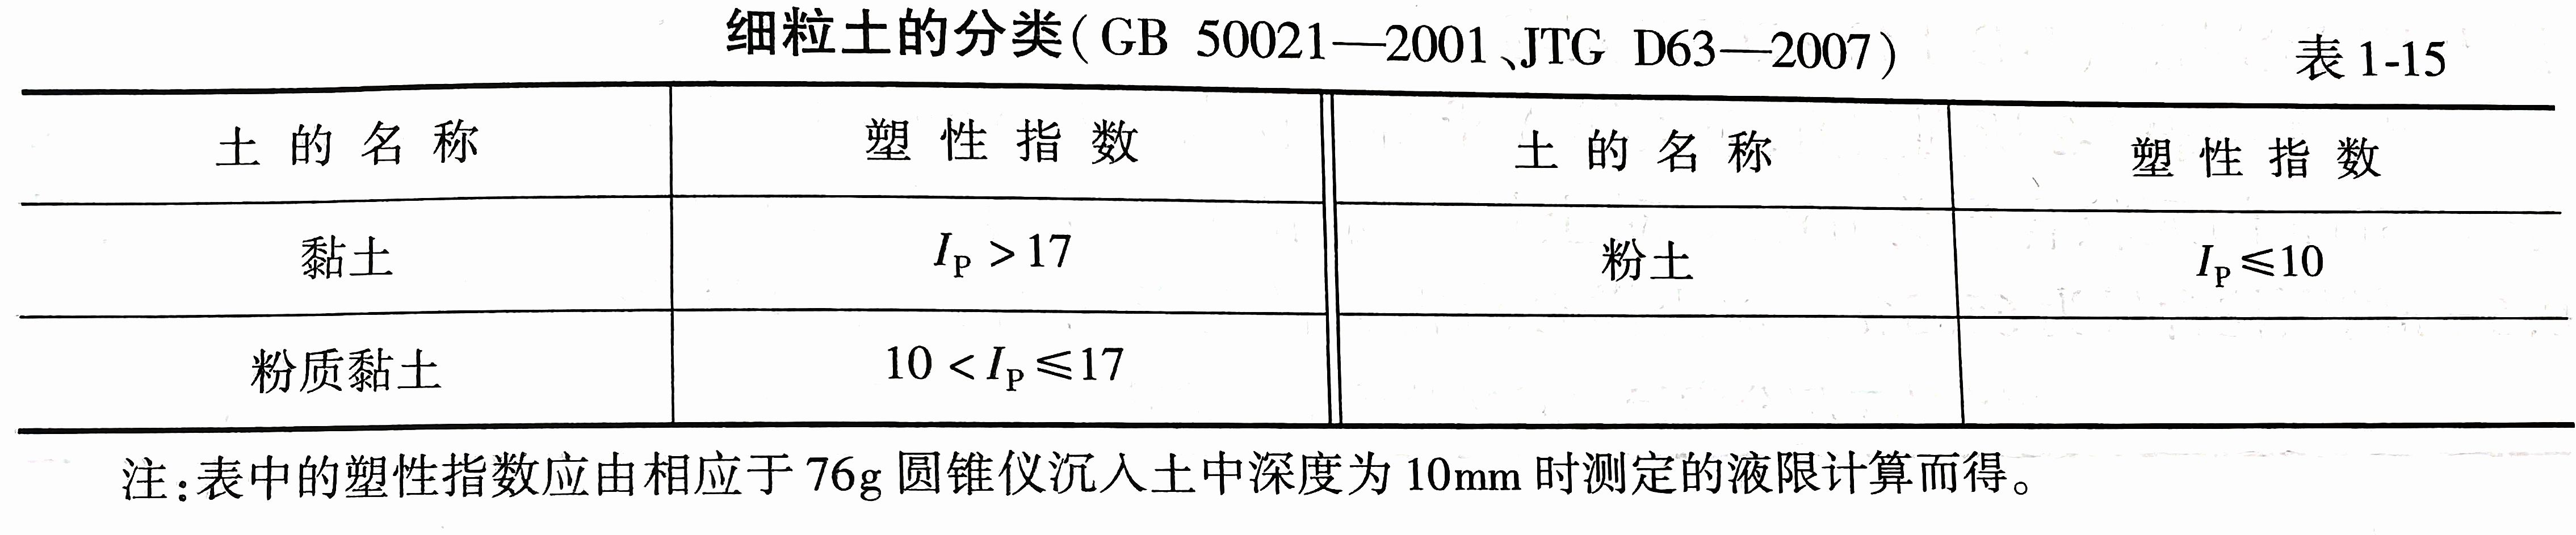
\includegraphics[width = 14cm ]{xltfl}
		\end{figure}
	
	\textcolor{cyan}{液性指数($I_L$)}:表示黏性土所处的软硬状态:
		\begin{equation}
			I_L=\frac{\omega - \omega_P}{I_P}=\frac{\omega - \omega_P}{\omega_L-\omega_P}
		\end{equation}
	
	可塑状态的土的液性指数在0\textasciitilde1之间,液性指数越大表示土越软;大于1表示土处于流动状态,小于0表示土处于固体状态或半固体状态。
	
	\subsection{无黏性土的密实度}
	\textcolor{cyan}{砂土的相对密实度}为:
		\begin{equation}
			D_r=\frac{e_{max}-e}{e_{max}-e_{min}}
		\end{equation}
	
	式中:
\begin{table}[h]
	\centering
	\begin{tblr}{|c|c|}
	\hline
	$e_{max}$&砂土最松散状态时的孔隙比,即最大孔隙比\\
	\hline
	$e_{min}$&砂土最密实状态时的孔隙比,即最小孔隙比\\
	\hline
	$e$&砂土在天然状态时的孔隙比。\\
	\hline
	\end{tblr}
\end{table}

	按照相对密度可分为三种密实度
\begin{figure}[H]%以后浮动体一律用figure,table太蛋疼了
	\centering
	\begin{tblr}{|c|c|c|c|}
		\hline
		密实度 & 密实 & 中密 & 松散\\
		\hline
		相对密度 & 1\textasciitilde0.67 & 0.67\textasciitilde0.33 & 0.33\textasciitilde0\\
		\hline
	\end{tblr}
\end{figure}

	\newpage 
                
	 
\section{第二章:黏性土的物理化学性质}
	没啥重点,看看书和习题册即可
	
	\section{第三章:土中水的规律}
	\subsection{土的渗透性}  
	\textcolor{cyan}{渗透}:在水位差的作用下,水透过土体空隙流动的现象
	  
	\textcolor{cyan}{水头}:任意断面处单位重量水的能量,等于比能(单位质量水的能量)除以重力加速度,单位为m
	
	\subsection{达西渗透定律}   
	在实际工程中不需要了解具体孔隙的渗流情况,因此可以对渗流做出如下简化:
	\begin{enumerate}
		\item 不考虑渗流路径的迂回曲折,只分析主要流向
		\item 不考虑土体中颗粒的影响,认为孔隙的土粒所占的空间的总和均为渗流所充满  
	\end{enumerate} 

	如图所示为简化的渗流模型:
	\begin{figure}[h]
		\centering
		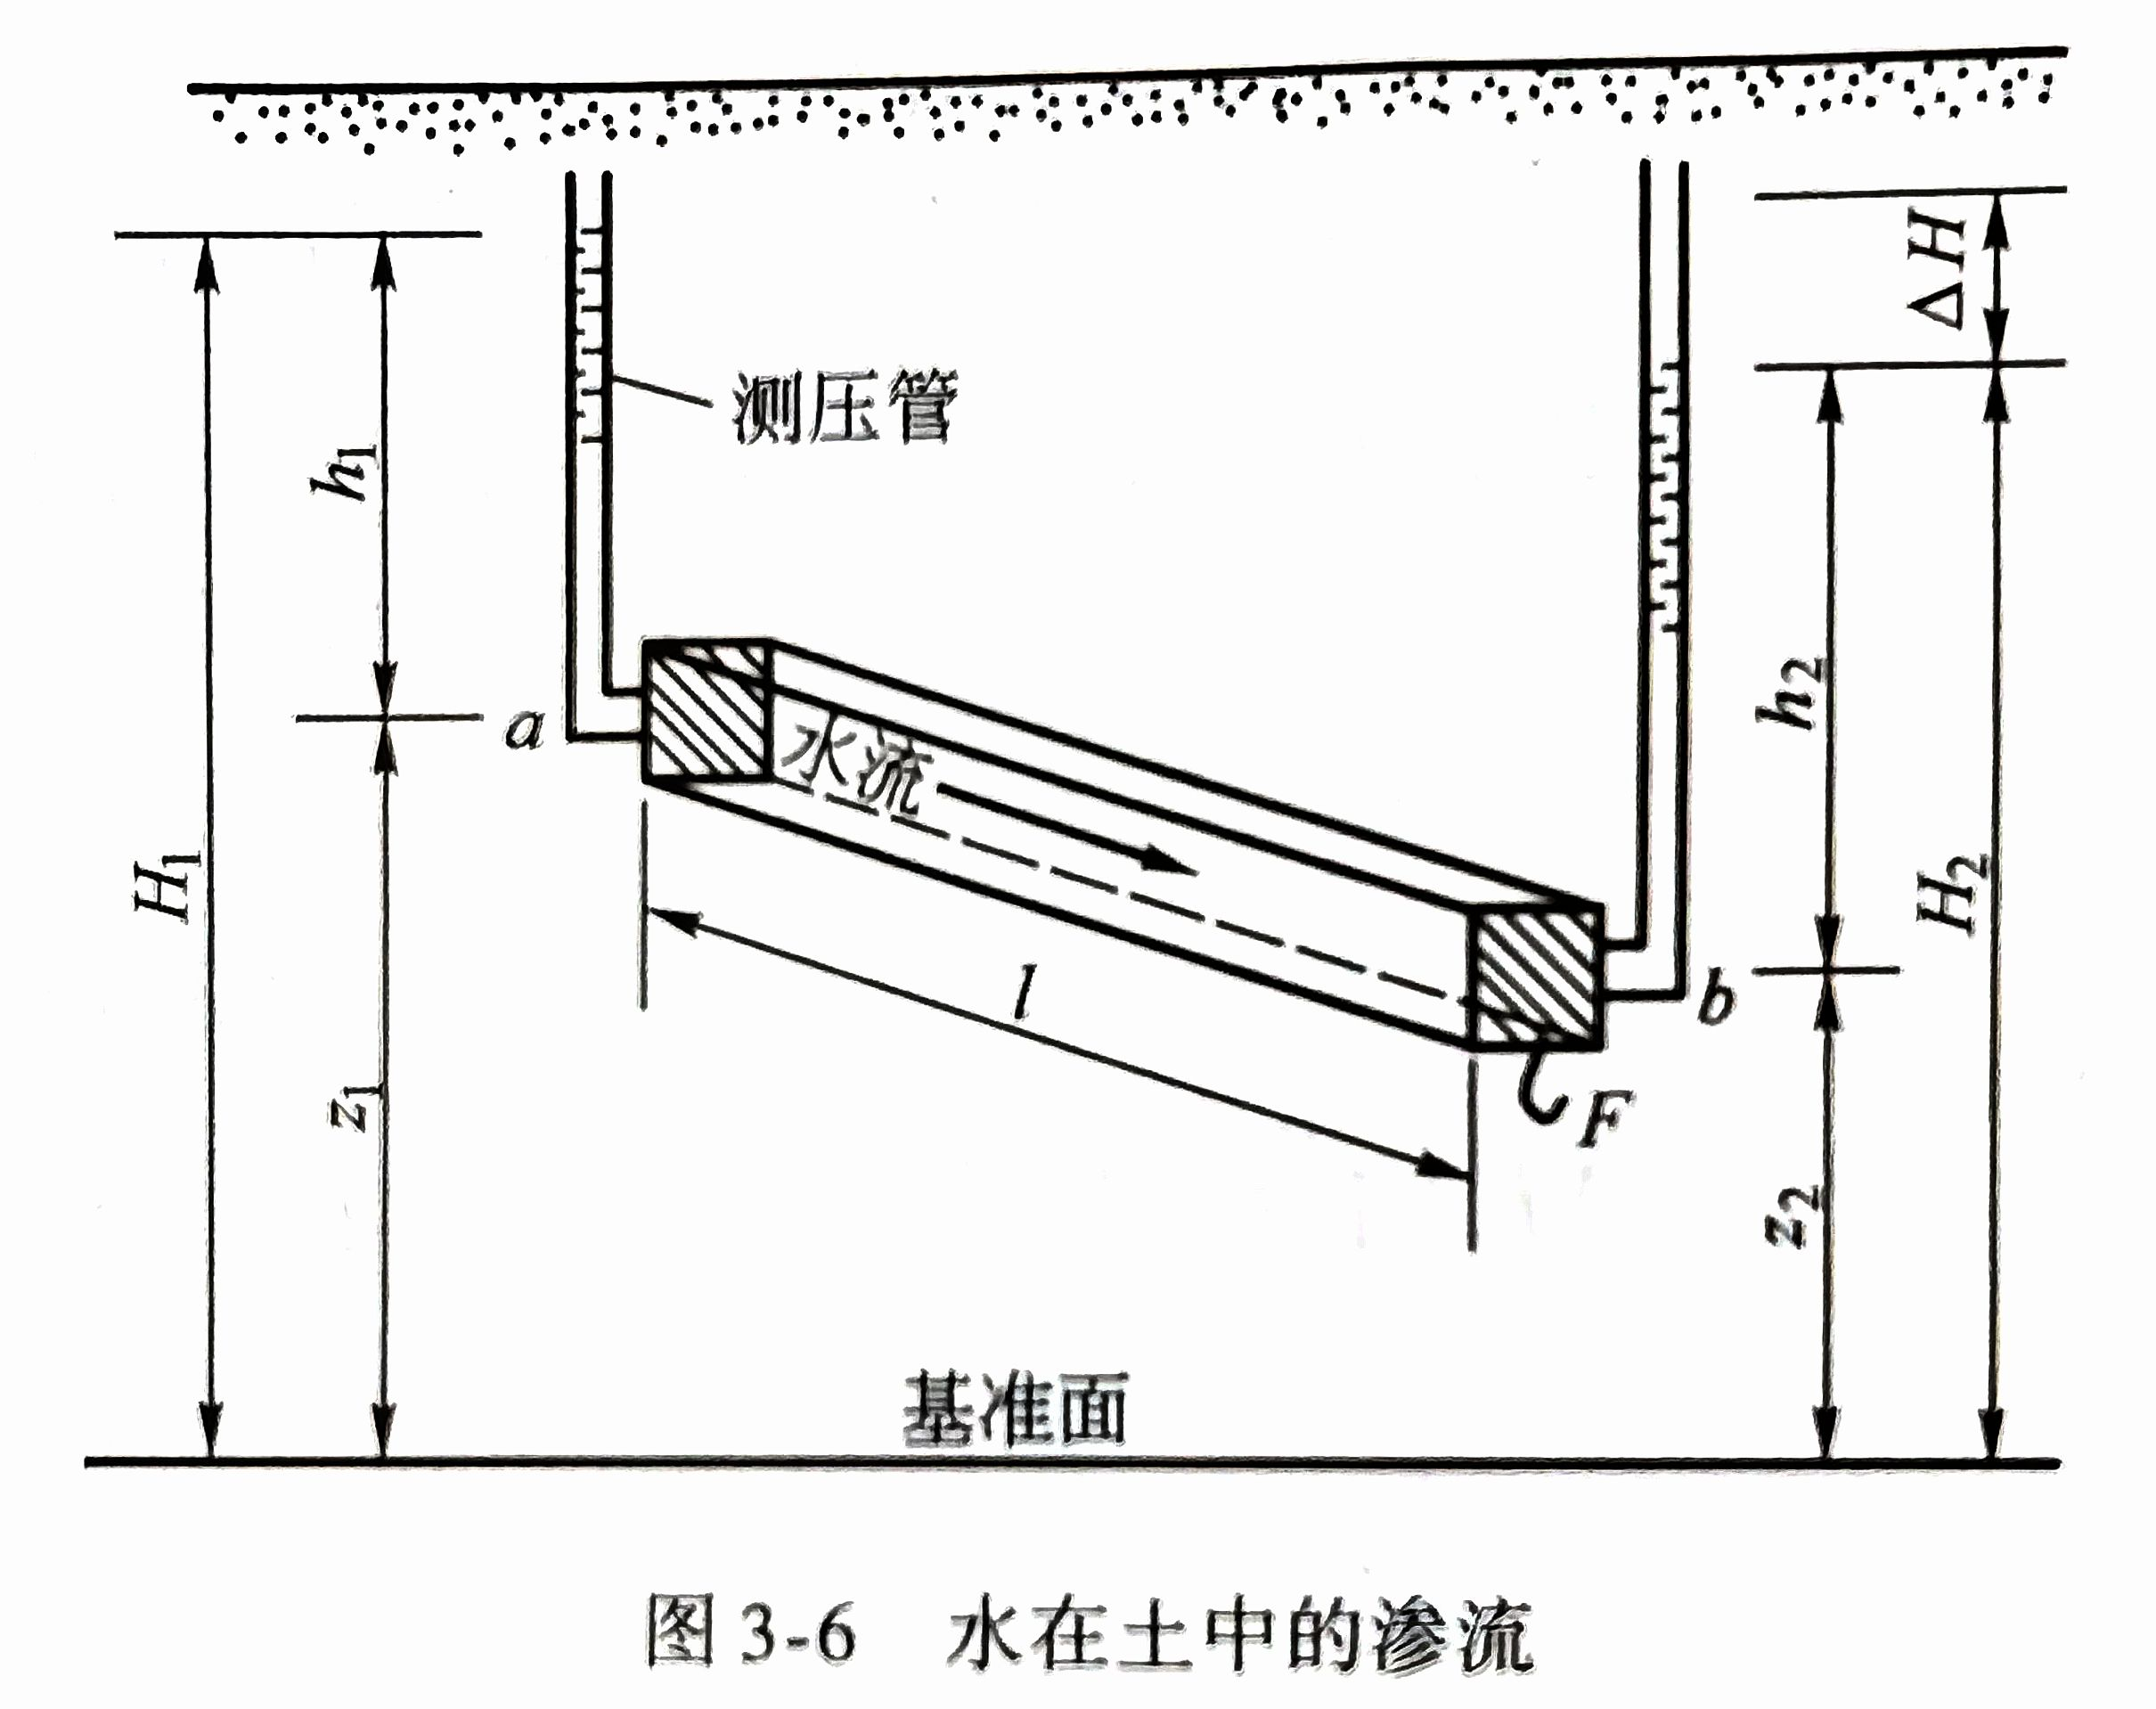
\includegraphics[width = 8cm ]{sl}
	\end{figure}

	\textcolor{cyan}{达西定律}的基本公式为: 
	\begin{gather}
			v=kI\\
			q=kIF
	\end{gather}
	
	其中:
	\begin{itemize}
		\item v为渗流速度($m/s$)
		\item I为水头梯度,即沿着水流方向单位长度上的水头差,如图中a、b两点的水头梯度为$I=\Delta H/\Delta l=(H_1-H_2)/l$
		\item k为渗透系数($m/s$)
		\item q为渗透流量($m^3/s$)
	\end{itemize}  

	注意:达西定律只适用于\textcolor{red}{\textbf{层流}}的情况,故一般只适用于中砂、细砂、粉砂等,不适用于粗砂,砾石、卵石等粗颗粒土。
	
	在t时间内流过土样的流量为Q,得:  
	\begin{equation}
		Q=qt=kIFt=k\frac{\Delta H}{l}Ft
	\end{equation}
	
	
	可得土样的渗透系数k为:
	\begin{equation}
		k=\frac{Ql}{\Delta HFt}
	\end{equation}
	
	 \subsection{动水力(渗透力)及渗流破坏}
	\textcolor{cyan}{动水力}:渗透水流施于单位土体内土粒上的拖拽力,大小与水力梯度成正比,作用方向与渗流方向一致,是一种\textcolor{red}{\textbf{体积力}}。  
	计算公式为:
	\begin{equation}
		G_D=T=\gamma_wI
	\end{equation}

	流土和管涌的区别如下表所示:
	
	\begin{figure}[H]%perfect LaTeX table!!!!!!
		\centering
		\begin{tblr}{|c|X|X|}
			\hline
			\diagbox{方面}{类别} & \SetCell{c} 流土 & \SetCell{c} 管涌 \\
			\hline
			\SetCell{c} 现象 & 土体局部范围的颗粒同时发生移动 & 土体内细颗粒通过粗粒形成的孔隙通道移动 \\
			\hline
			\SetCell{c} 位置 & 只发生在水流渗出的表层,由自下而上的渗流引起 & 可发生于土体内部和渗流溢出处,水平渗流可引起 \\
			\hline
			\SetCell{c} 土类 & 只要渗透力足够大,可发生在任何土中 & 一般发生在特定级配的无黏性土或分散性黏土 \\
			\hline
			\SetCell{c} 历时 & 破坏过程时间短 & 破坏过程为时长 \\
			\hline
			\SetCell{c} 后果 & 导致下游坡面产生局部滑动 & 导致结构发生塌陷或渍口 \\
			\hline
		\end{tblr}
	\end{figure}
	
	\textcolor{cyan}{流砂现象}:当向上的动水力$G_D$与土的有效重度$\gamma'$相等时,即
	\begin{equation}
		G_D=\gamma_wI=\gamma'=\gamma_{sat}-\gamma_w
	\end{equation}
	
	由上式知:
	\begin{equation}
		I=\frac{\gamma'}{\gamma_w}=\frac{\gamma_{sat}-\gamma_w}{\gamma_w}=I_{cr}
	\end{equation}

	此时的水头梯度称为\textcolor{cyan}{临界水头梯度$I_{cr}$},\textcolor{red}{\textbf{发生流沙的条件}}即为$I>I_{cr}$。
	
	\subsection{一句可能有用的话}
	\textcolor{cyan}{冻胀现象}常发生在细粒土中,特别是\textcolor{red}{\textbf{粉土、粉质粘土中}},冻结时水分迁移积聚最为强烈,冻胀现象严重。
	
	\newpage
	
\section{第四章:土中应力计算}
	\textcolor{cyan}{土的应力}包括\textbf{自重应力}和\textbf{附加应力},前者是因土受到重力作用而产生的;后者是因受到建筑物等外荷载作用而产生的。
	
	\subsection{土的自重应力计算}
	如图所示为土中应力分布:
	\begin{figure}[h]
		\centering
		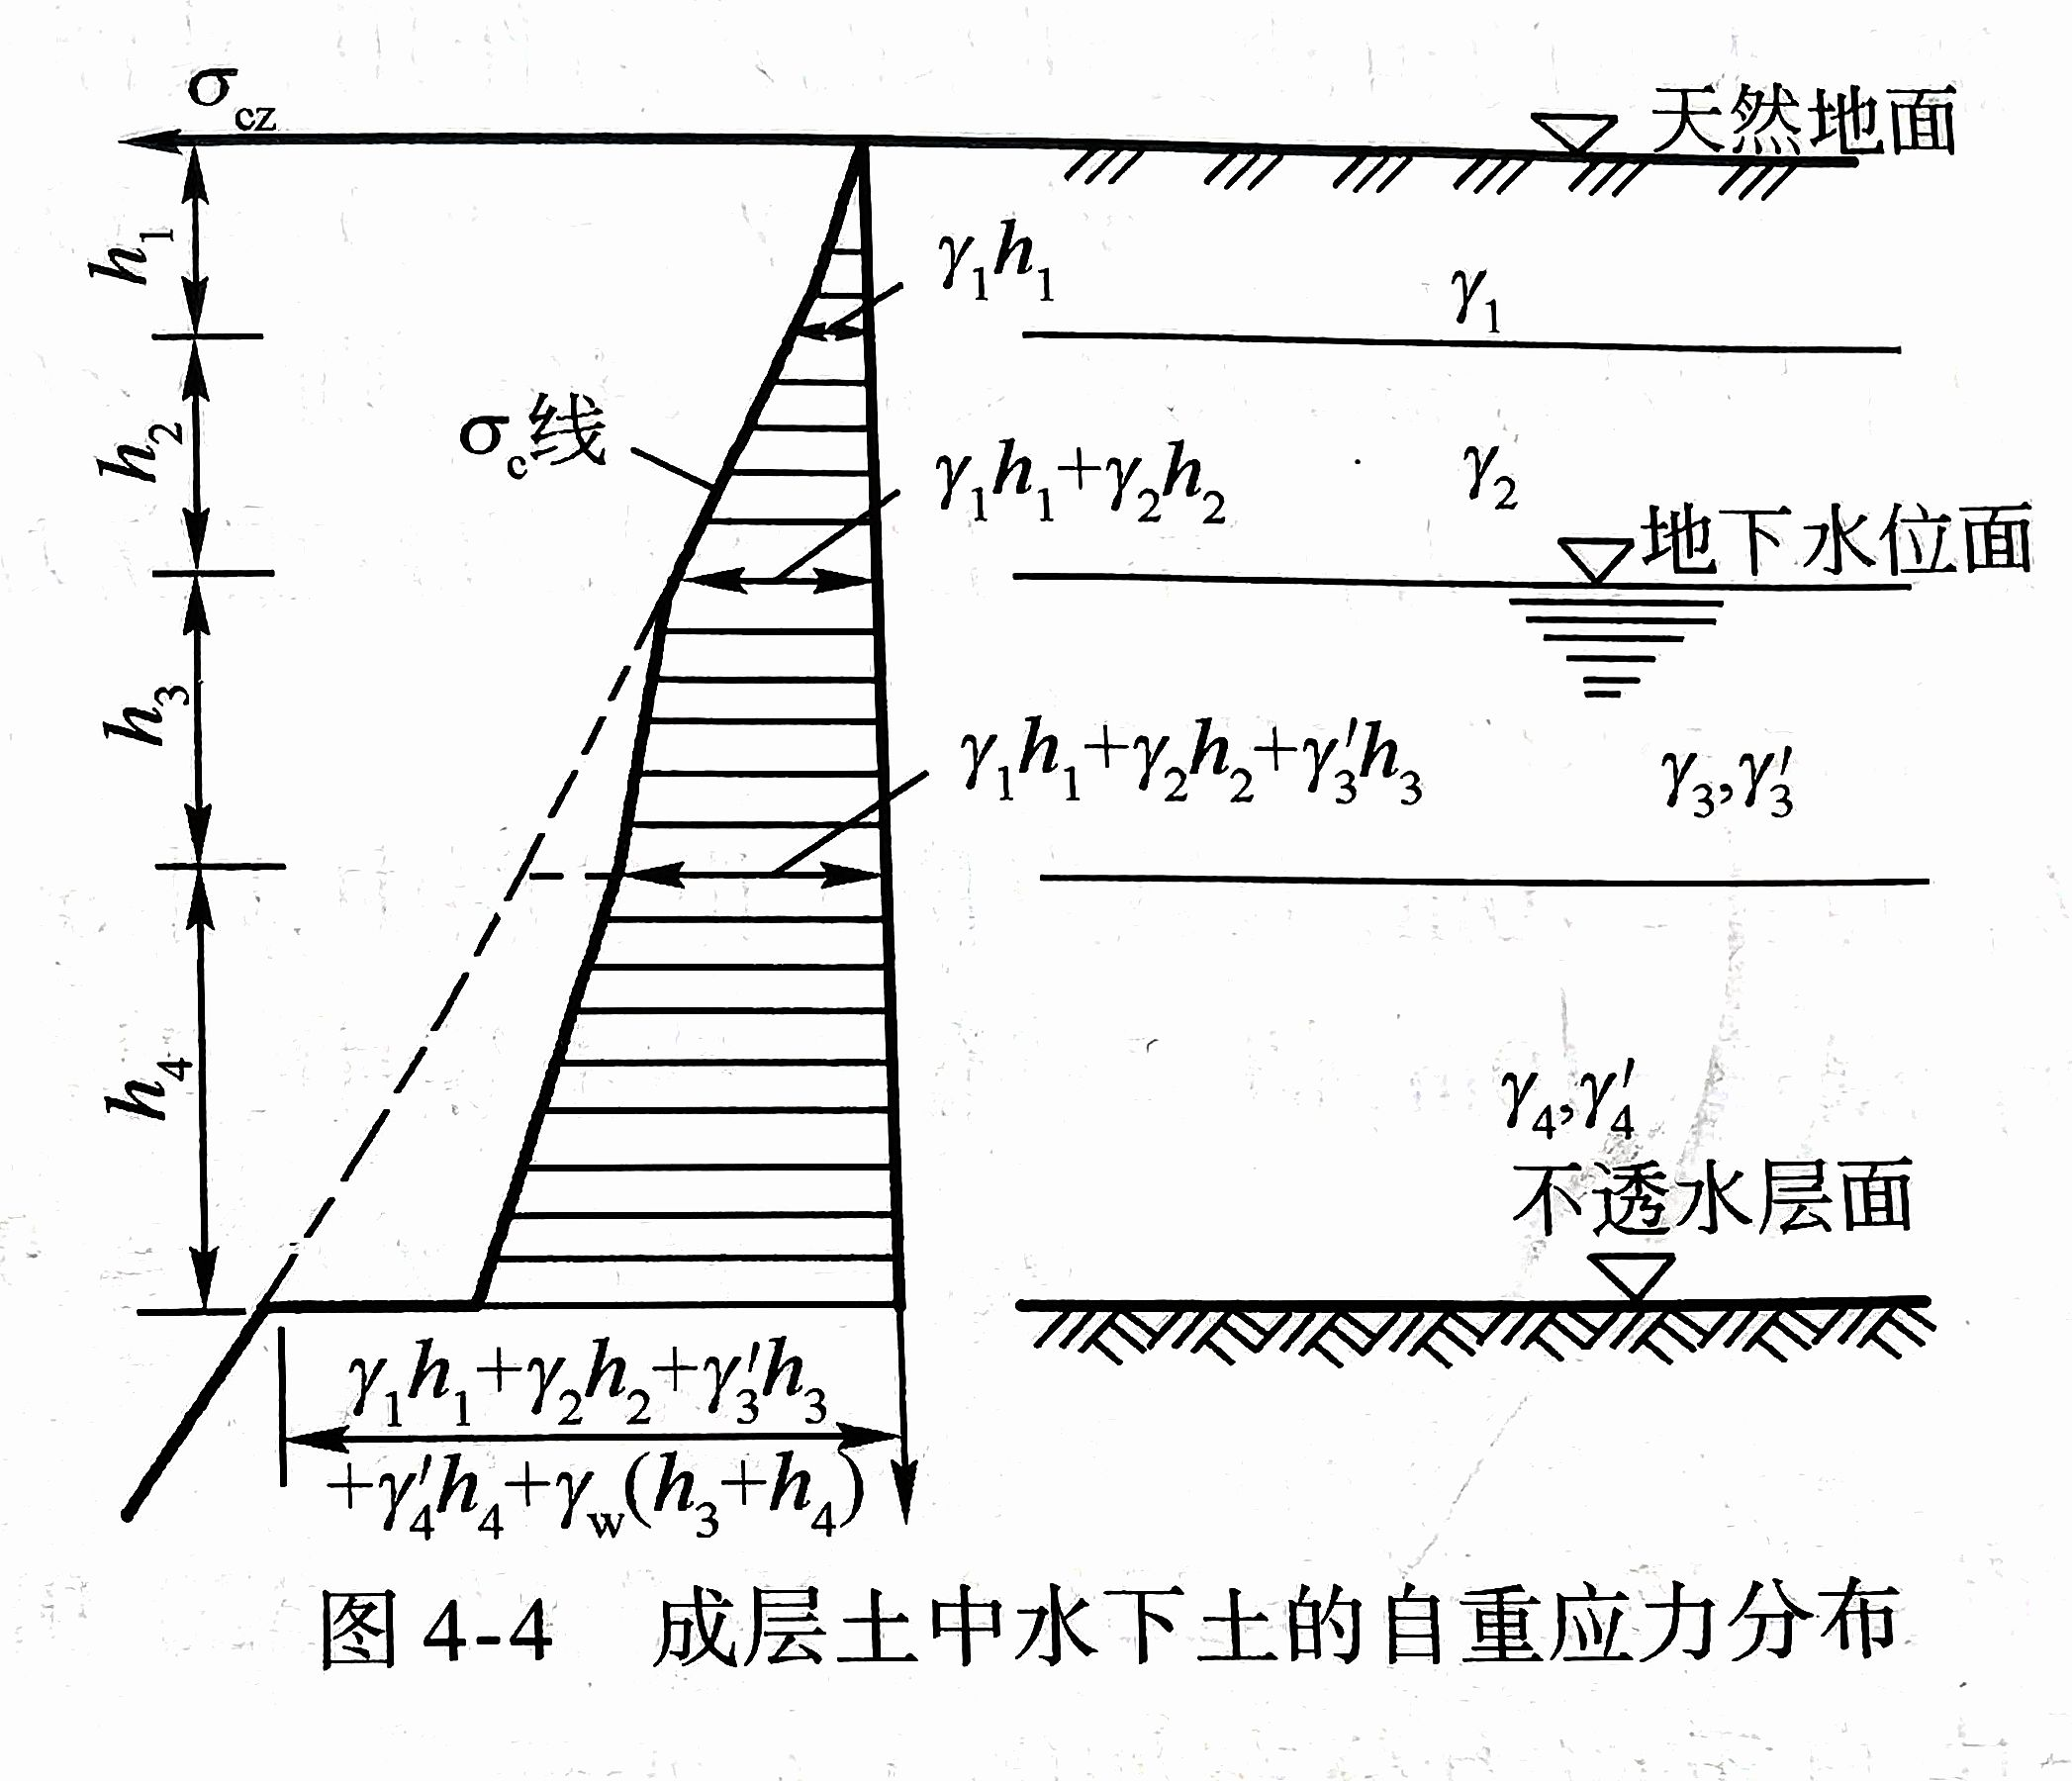
\includegraphics[width = 6cm ]{ylfb}
	\end{figure}
	
	自重应力计算公式为:
	\begin{equation}
		\sigma_{cz}=\gamma_1h_1+\gamma_2h_2+\gamma_3h_3+\cdots \gamma_nh_n=\sum_{i=1}^{n} \gamma_ih_i
	\end{equation}

	注意:对于水位以下土的自重应力,应考虑是否受水的浮力作用,具体重度取值($\gamma$)情况如下:
	\begin{figure}[h]
		\centering
		\begin{tblr}{|c|c|c|c|}
			\hline
			砂性土 & \SetCell[c=3]{c} 取有效重度$\gamma'$ & & \\
			\hline
			\SetCell[r=2]{c} 黏性土 & $I_L\geqslant 1$ & 流动状态 & 取有效重度$\gamma'$ \\
			\hline
			 & $I_L\leqslant 0$ & 固体状态 & 取天然重度$\gamma$ \\
			\hline 
		\end{tblr}
	\end{figure}

	\subsection{基底压力的简化计算方法}
	如图所示为基底压力的两种情况:\textcolor{cyan}{中心荷载}及\textcolor{cyan}{偏心荷载}:
	\begin{figure}[H]
		\centering
		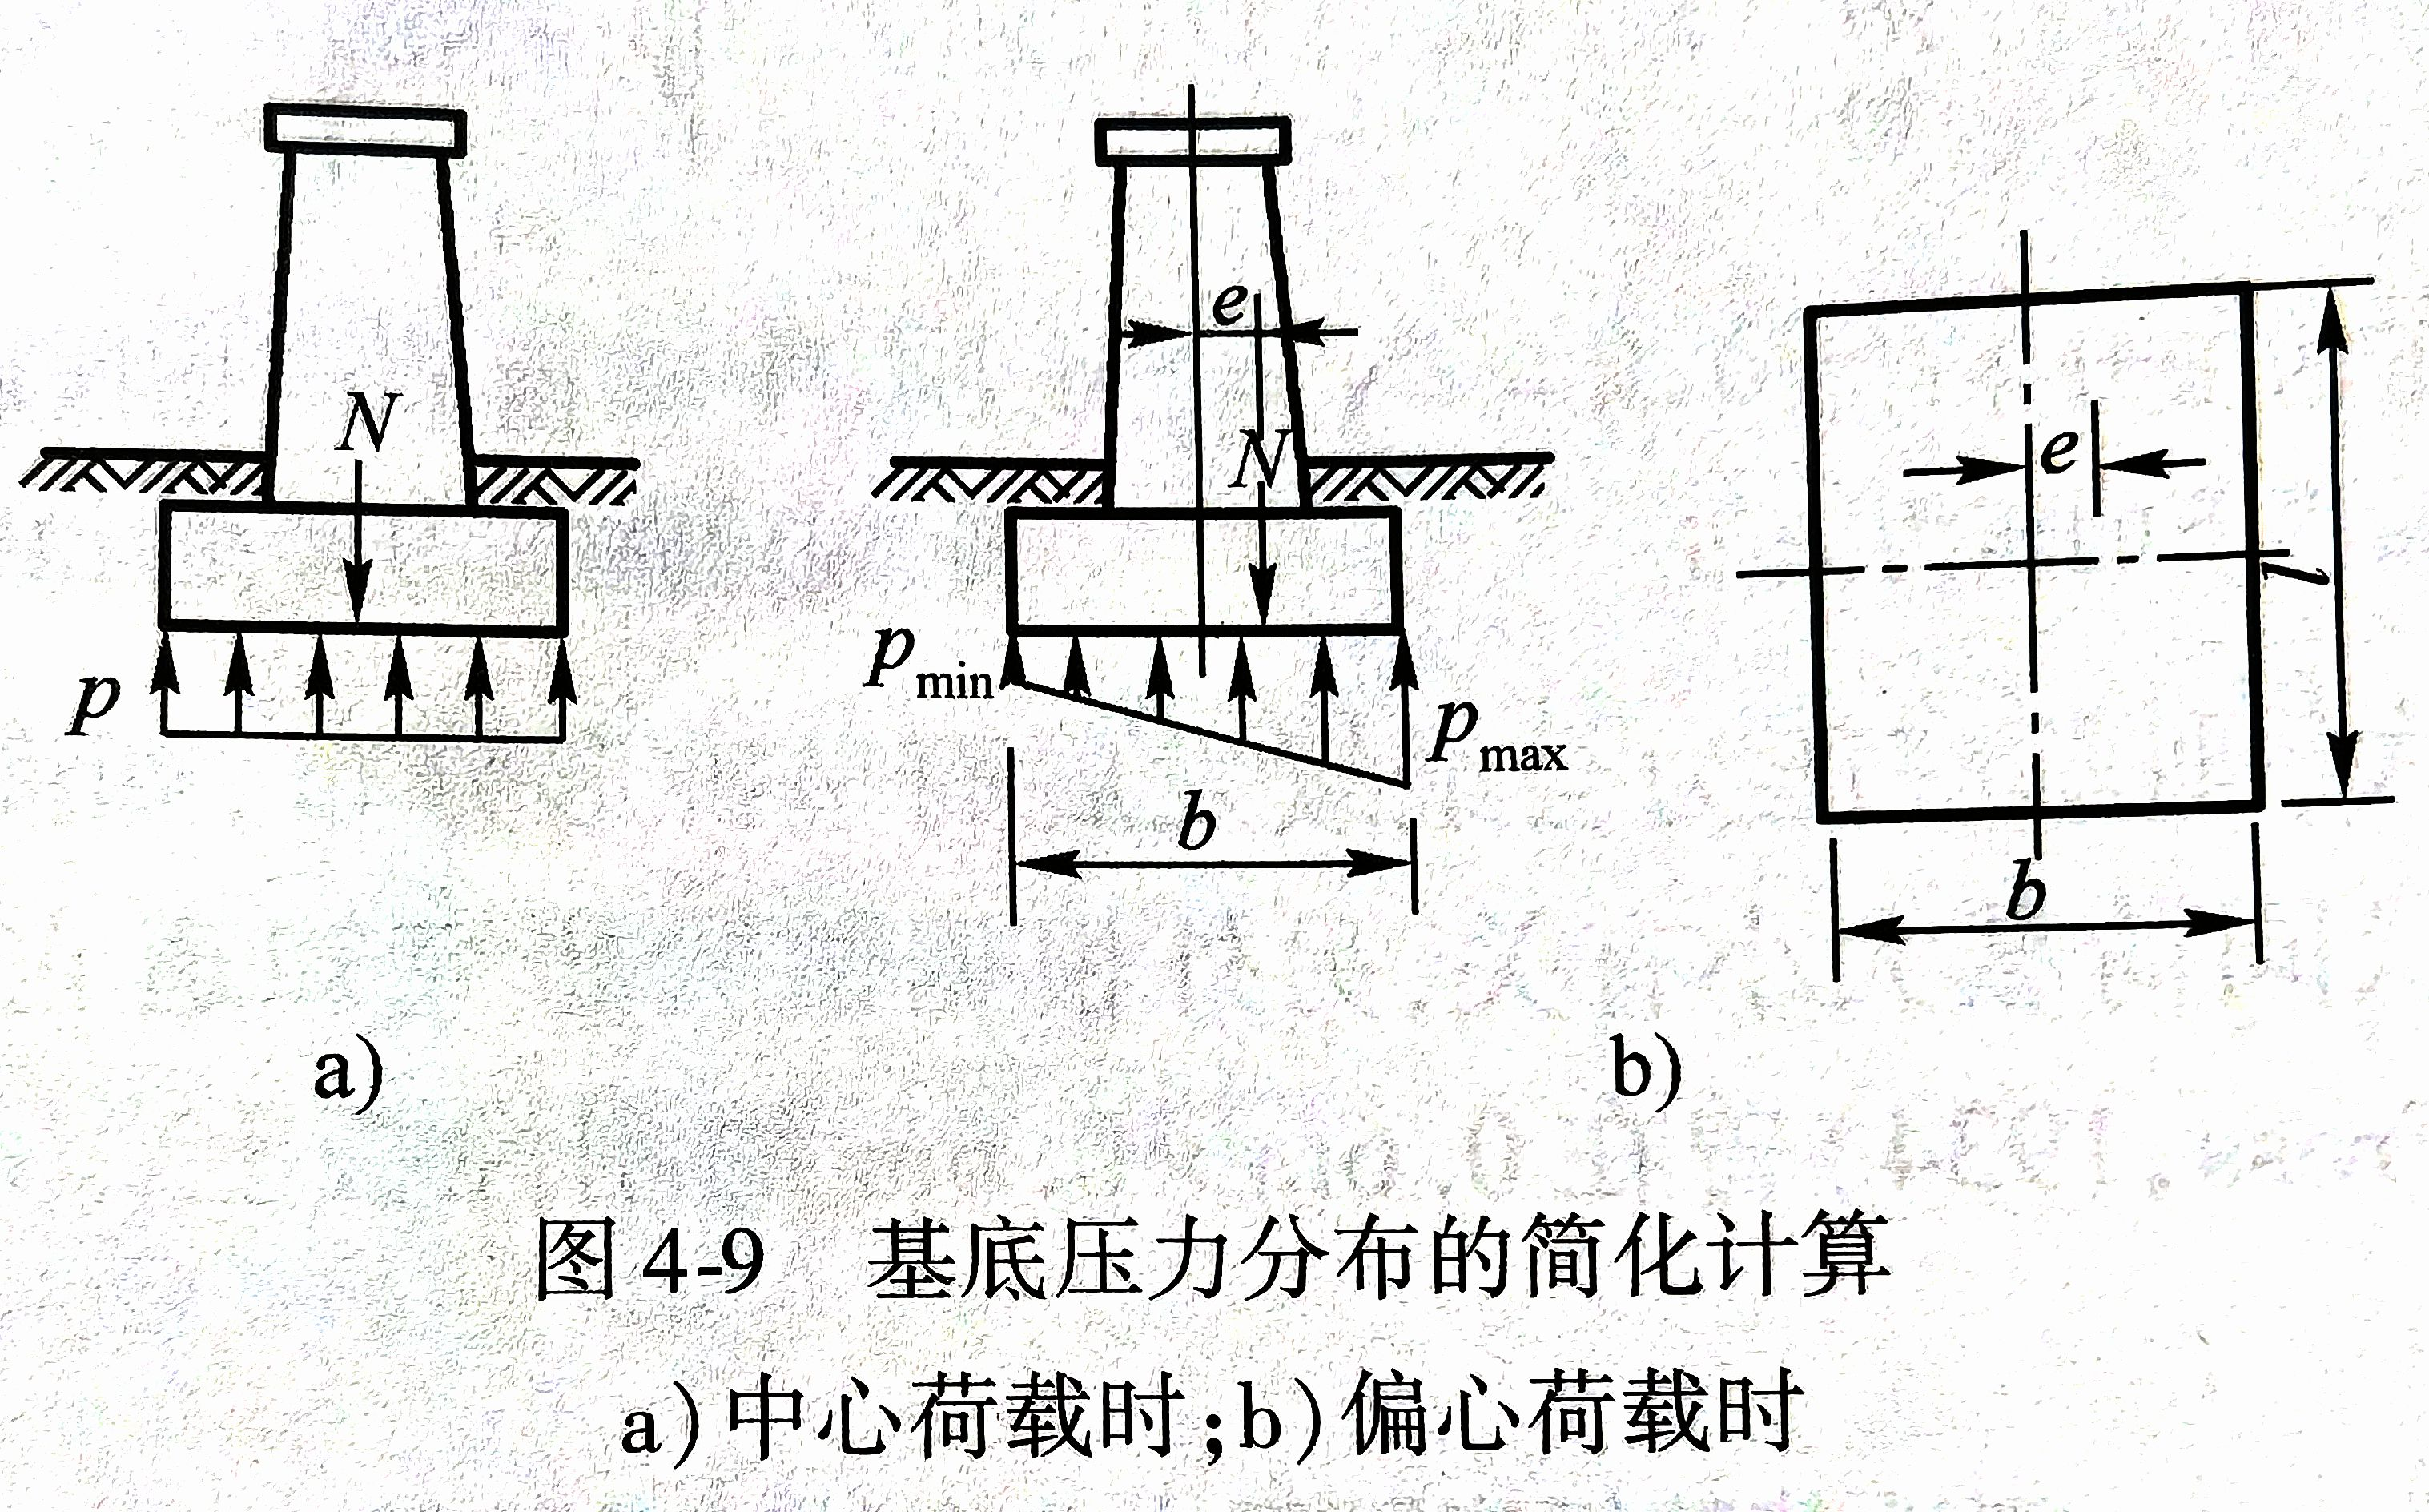
\includegraphics[width = 6.3cm ]{zxpx}
	\end{figure}

	\noindent\textbf{1. 中心荷载}
	
	基底压力$p$为:
	\begin{equation}
		p=\frac{N}{F}
	\end{equation}

	式中:
	\begin{itemize}
		\item $N$为作用于基础底面中心的竖直荷载
		\item $F$为基础底面积
	\end{itemize}

	\noindent\textbf{2. 偏心荷载}
	
	偏心受压公式为:
	\begin{equation}
		p_{min}^{max}=\frac{N}{F}\pm \frac{M}{W}=\frac{N}{F}(1\pm \frac{6e}{b})
		\label{px}
	\end{equation}
	
	式中:
	\begin{itemize}
		\item $N$、$M$分别为作用在基础底面中心的竖直荷载及弯矩,$M=Ne$
		\item $e$为荷载偏心距(在宽度$b$方向上)
		\item $W$为基础底面的抵抗矩,对矩形基础$W=lb^2/6$
		\item $b$、$l$为基础底面的宽度与长度
	\end{itemize}
	
	按照偏心距$e$的大小,可将基底压力分布分为三种情况:
	\begin{figure}[H]
		\centering
		\begin{minipage}[c]{0.3\textwidth}
			\centering
			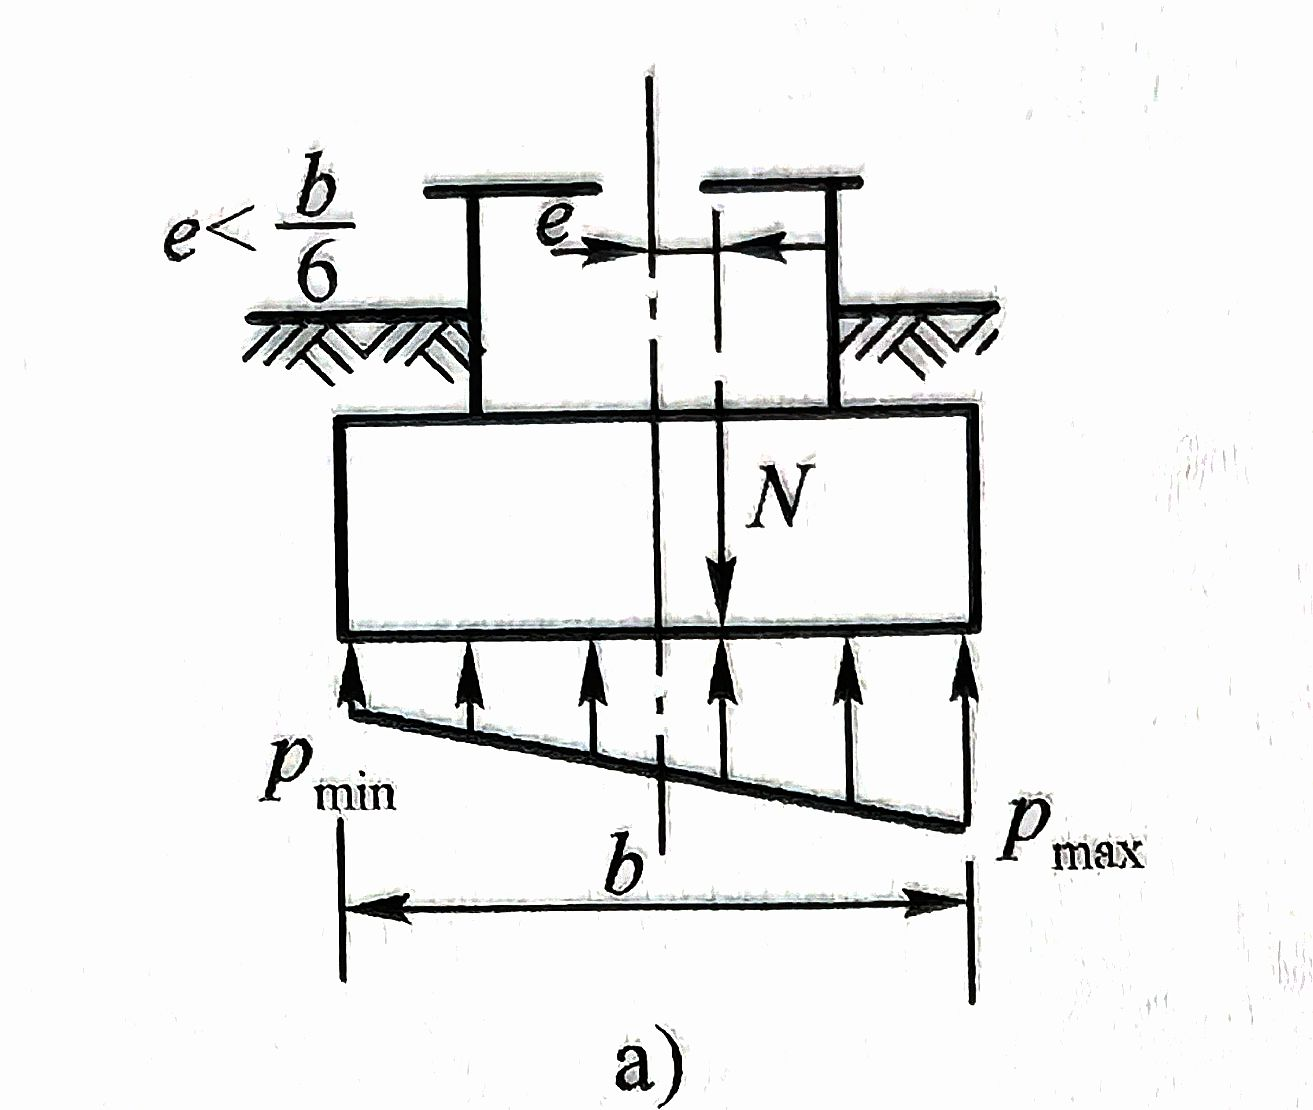
\includegraphics[width=1.1\textwidth]{a}
		\end{minipage}
		\begin{minipage}[c]{0.3\textwidth}
			\centering
			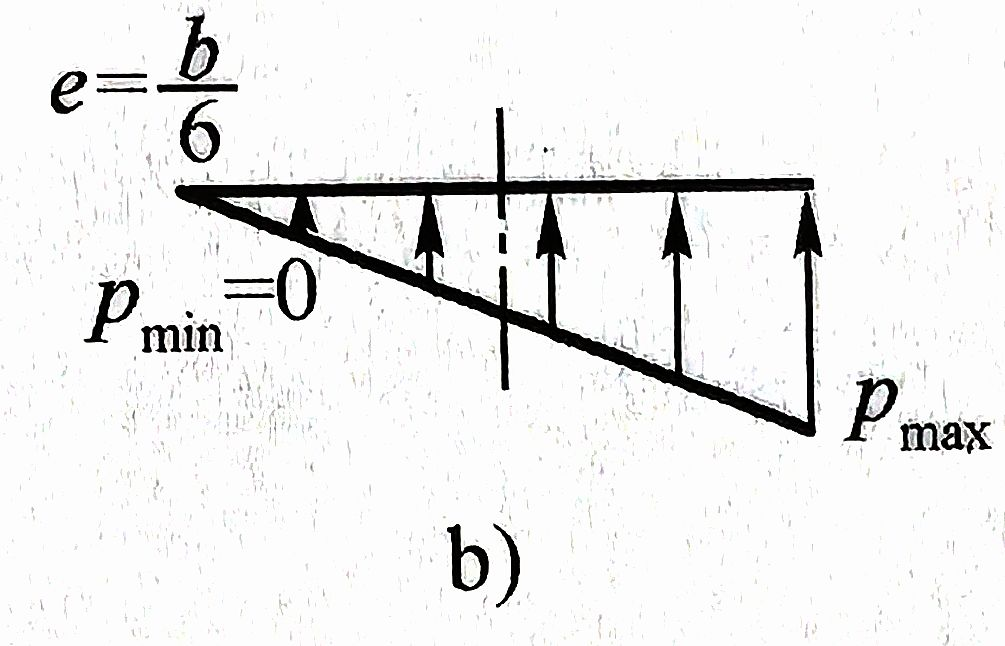
\includegraphics[width=1.1\textwidth]{b}
		\end{minipage}
	\end{figure}

	\begin{figure}[H]
		\centering
		\begin{minipage}[c]{0.3\textwidth}
			\centering
			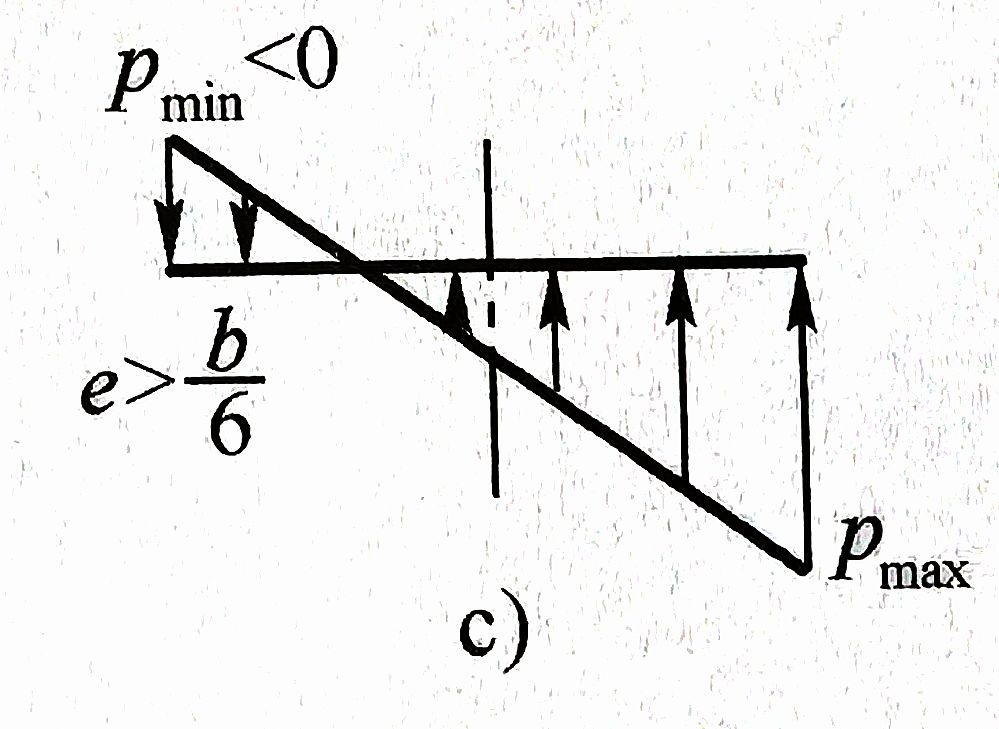
\includegraphics[width=1.1\textwidth]{c}
		\end{minipage}
		\begin{minipage}[c]{0.3\textwidth}
			\centering
			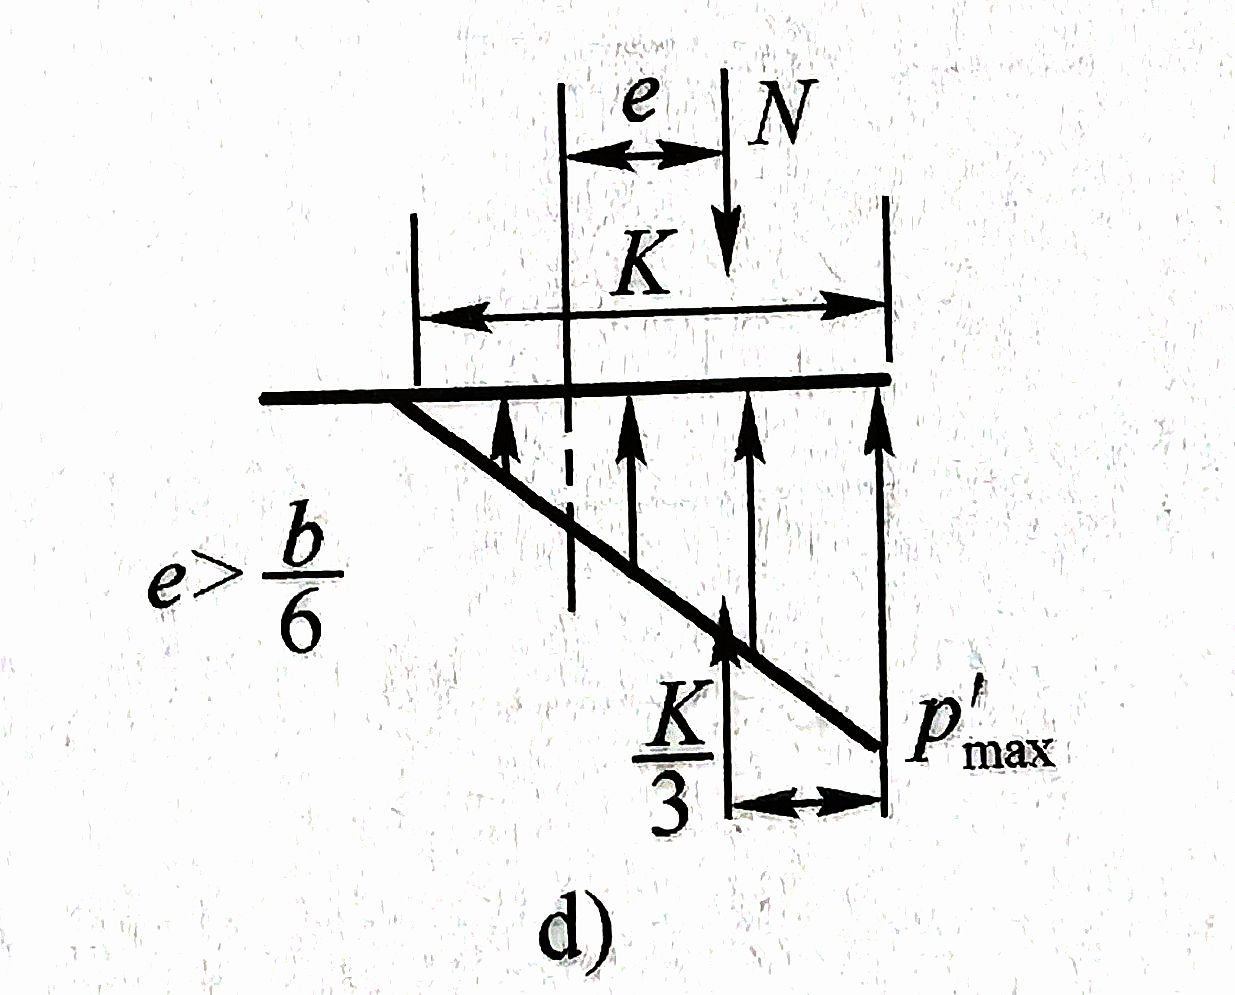
\includegraphics[width=1.1\textwidth]{d}
		\end{minipage}
	\end{figure}

	\begin{enumerate}
		\item 当$e<b/6$时,由公式\ref{px}知$p_{min}>0$,基底压力呈梯形分布,如图a所示
		\item 当$e=b/6$时,$p_{min}=0$,基底压力呈分布,如图b所示
		\item 当$e>b/6$时,$p_{min}<0$,也即产生拉应力(如图c),但是基底与土之间是无法承受拉应力的,基底压力会重新分布,重新分布后的最大压应力$p'_{max}$为
		\begin{equation}
			p'_{max}=\frac{2N}{3(\frac{b}{2}-e)l}
		\end{equation}
	\end{enumerate}
	  
	\subsection{竖向分布荷载作用下土中应力计算}
	一般计算矩形面积均布荷载作用,分为两种情况:
	
	\noindent\textbf{1.矩形面积中点$O$下土中竖向应力$\sigma_z$计算}
	
	如图所示:
	\begin{figure}[H]
		\centering
		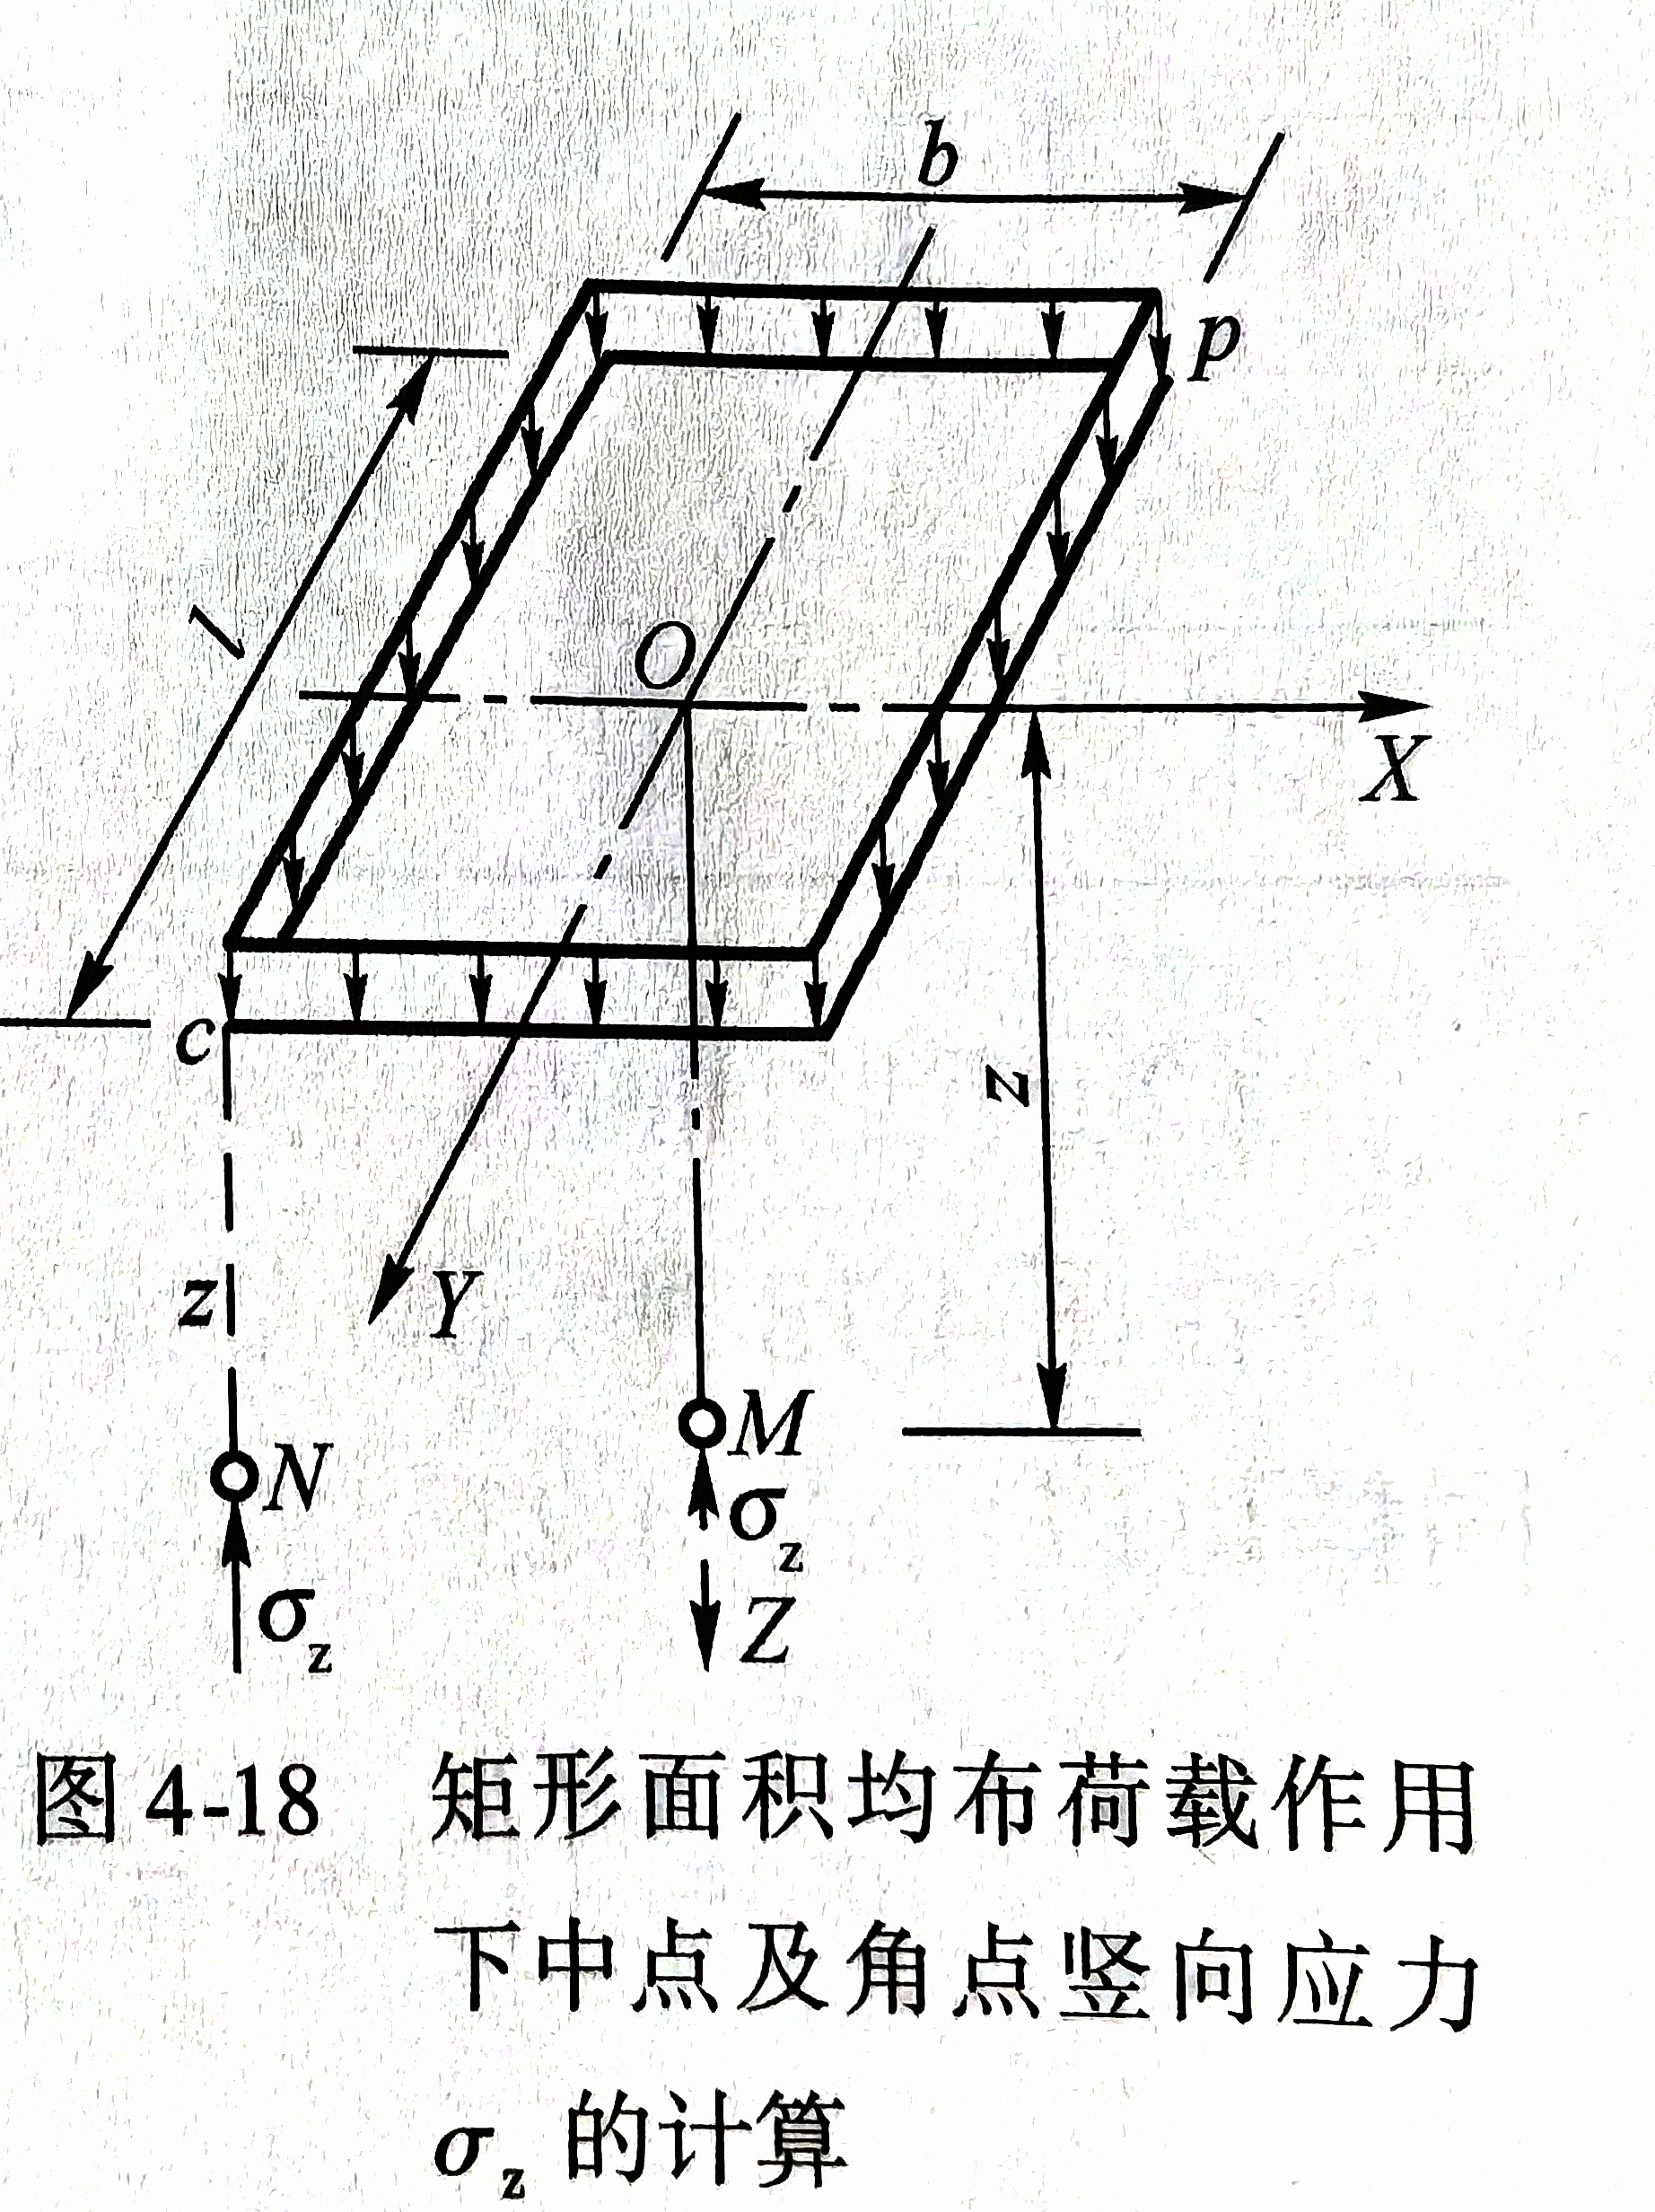
\includegraphics[width = 5cm ]{zd}
	\end{figure}
	
	大小为:
	\begin{equation}
		\sigma_z=\alpha_0p
	\end{equation}
	  
	其中$\alpha_0$可通过$n=l/b$、$m=z/b$查表得。
	
	\noindent\textbf{2.矩形面积下土中任一点的竖向应力$\sigma_z$计算————角点法}
	
	如图所示:
	\begin{figure}[H]
		\centering
		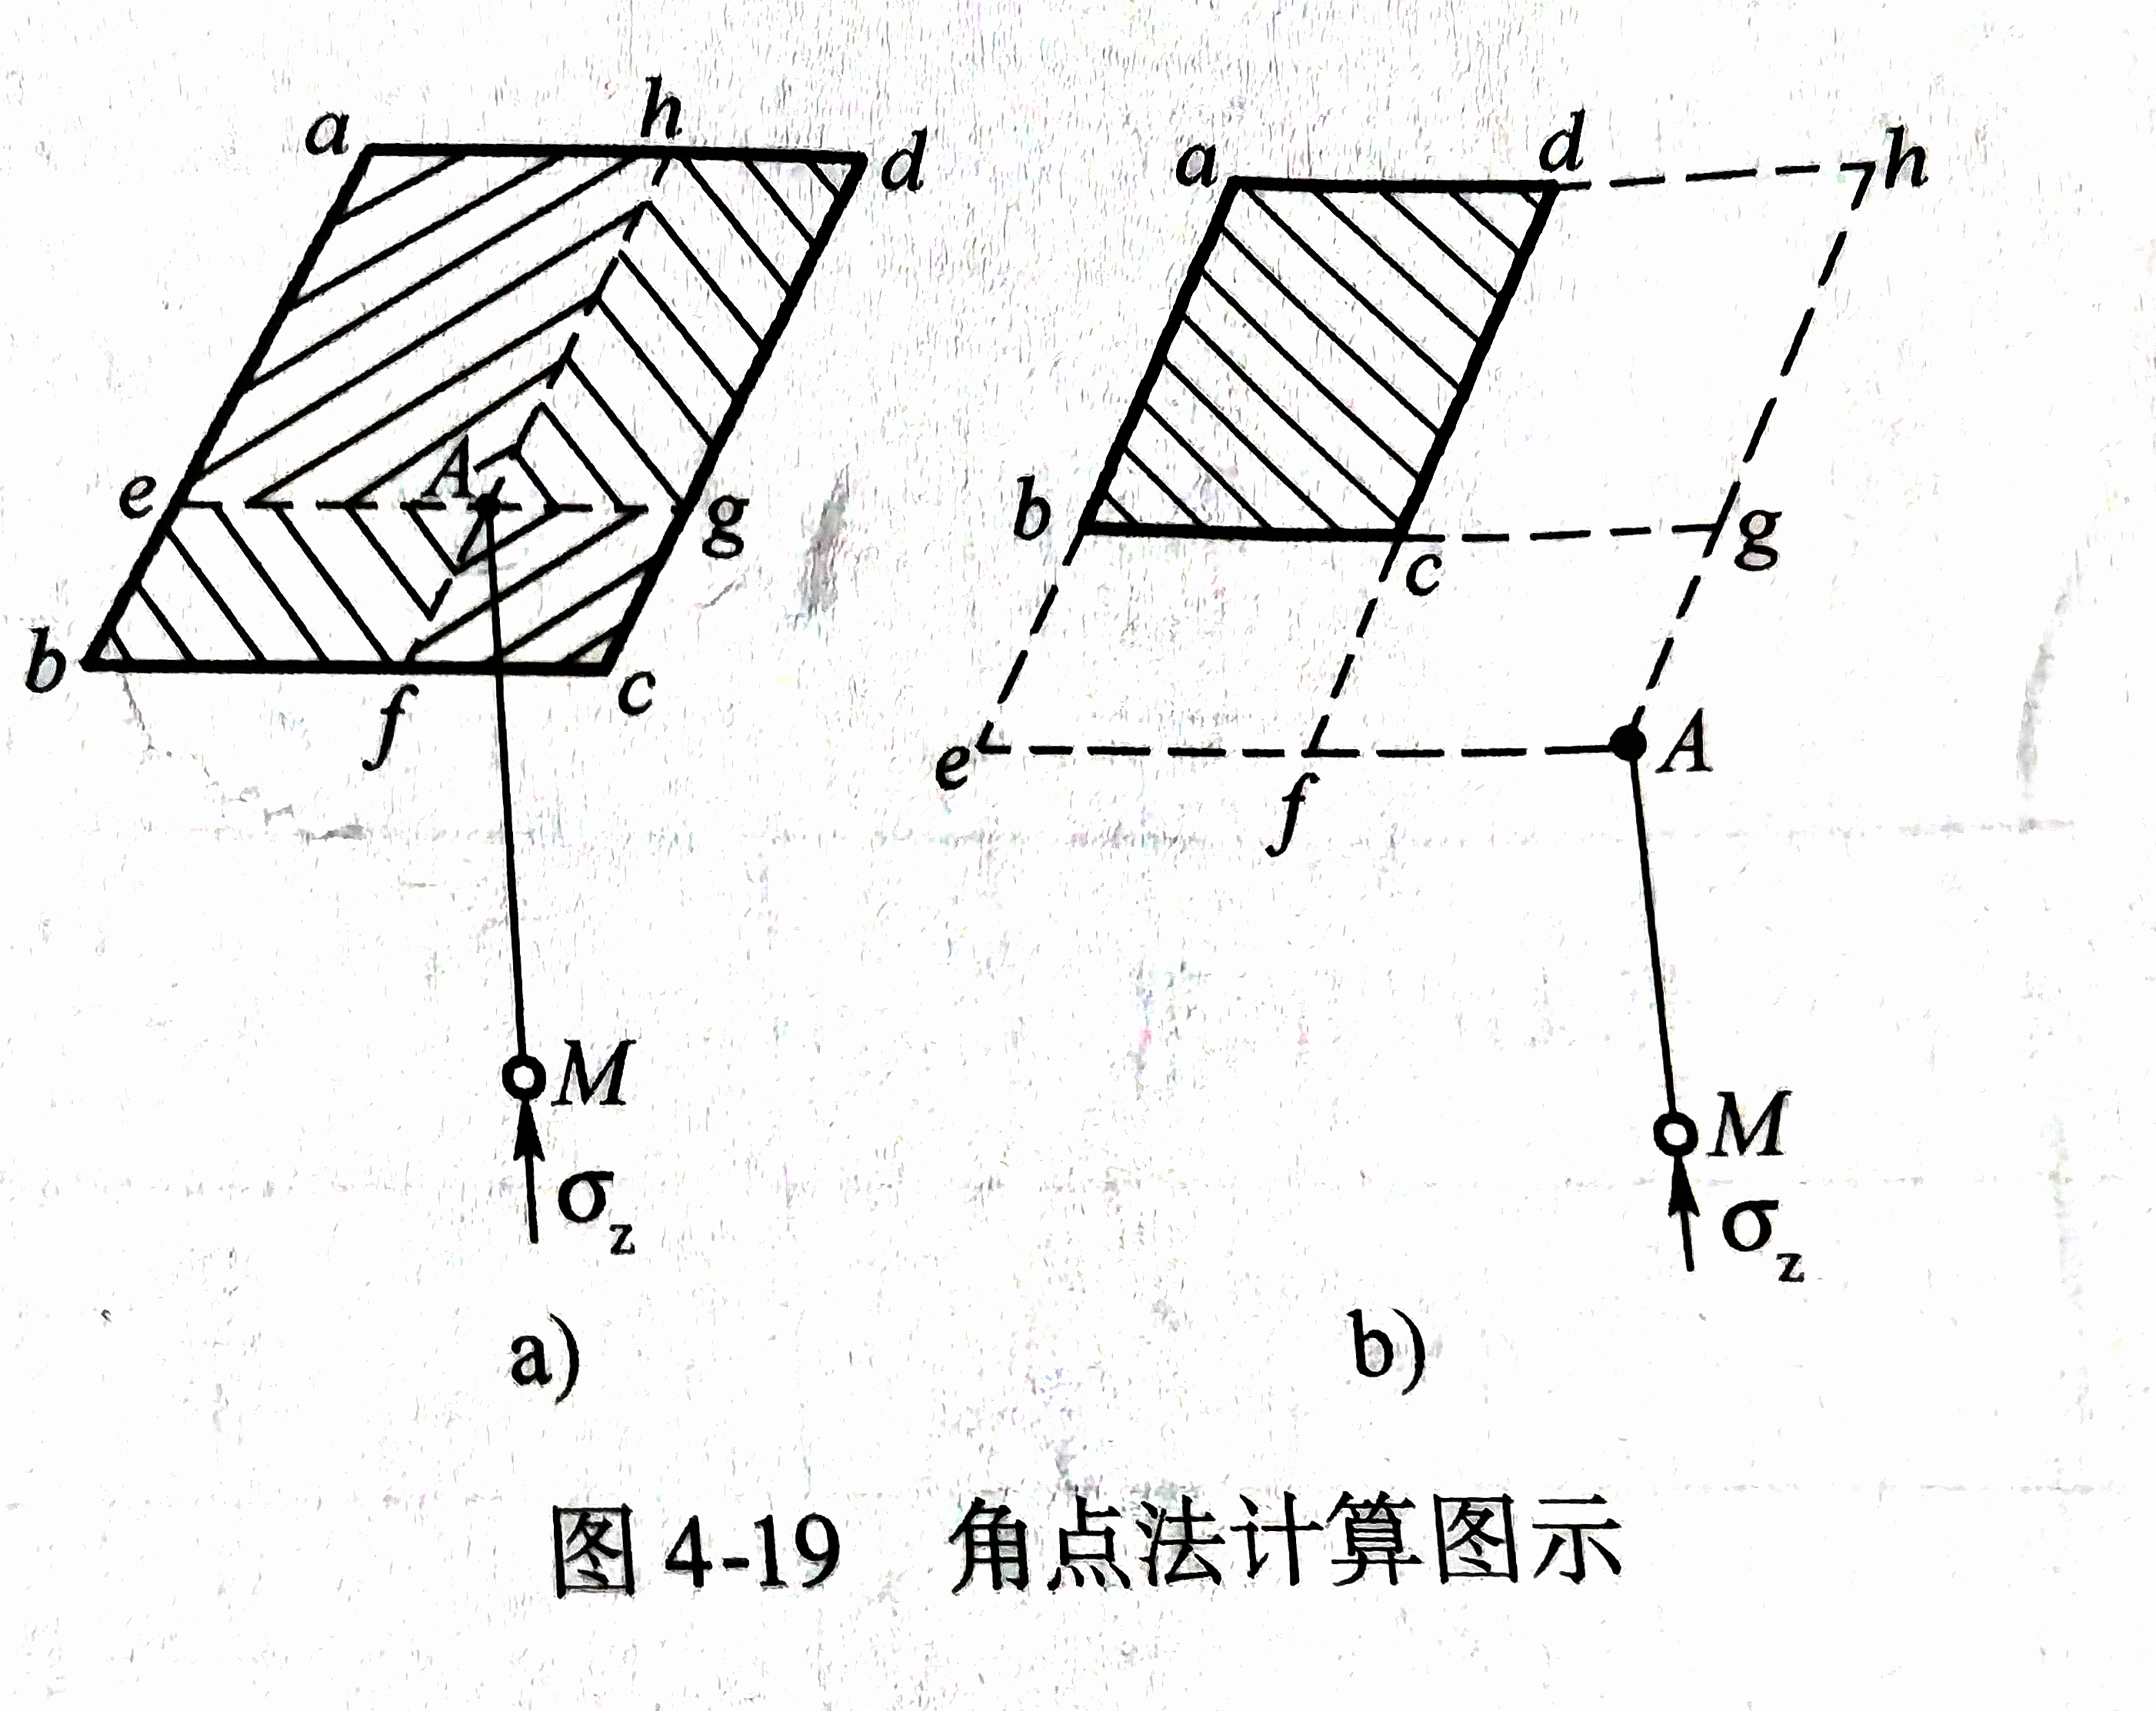
\includegraphics[width = 6cm ]{jdf}
	\end{figure}
	
	计算时可以通过$A$点将受荷面积$abcd$分为4个小矩形面积$aeAH$、$ebfA$、$hAgd$及$Afcg$,再分别计算4个小矩形面积均布荷载在角点$A$下引起得竖向应力$\sigma_{zi}$,再叠加即得(如图a):
	\begin{equation}
		\sigma_z=\sum\sigma_{zi}=\sigma_{z(aeAh)}+\sigma_{z(ebfA)}+\sigma_{z(hAgd)}+\sigma_{z(Afcg)}
	\end{equation}

	若A点在矩形面积范围之外(如图b),缺失部分减掉即可,即:
	\begin{equation}
		\sigma_z=\sum\sigma_{zi}=\sigma_{z(aeAh)}-\sigma_{z(ebfA)}-\sigma_{z(hAgd)}-\sigma_{z(Afcg)}
	\end{equation}
	
	同样,$\alpha_z$可通过$n=l/b$、$m=z/b$查表得。
	
	\subsection{饱和土有效应力原理}
	公式为:
	\begin{equation}
		\sigma=\sigma'+u
	\end{equation}

	两个要点:
	\begin{enumerate}
		\item 土的有效应力$\sigma'$等于总应力$\sigma$减去孔隙水压力$u$
		\item 土的有效应力控制了土的变形及强度性能
	\end{enumerate}

	
	
	
	
	
	
	
	
	
	\newpage
	%参考文献
	\bibliographystyle{unsrt}%这个style根据引用顺序,plain根据作者姓名排序
	
	\bibliography{document}
\end{document}